

% ---------------------------------------------------------------------------- %
% Pre

% Document
\documentclass[10pt, preprint]{sigplanconf}

% Standard
\usepackage{hyperref}
\usepackage[pass,letterpaper]{geometry}

% Libraries for drawing
\usepackage{graphicx}
\usepackage{mathptmx}
\usepackage[rgb]{xcolor}
\usepackage{pgfplots}
% \usepackage[subpreambles=true]{standalone}

% Custom
\usepackage{config/toggles}
\usepackage{config/terminology}
\usepackage{config/settings}

% Meta
% \usepackage[bookmarks=true,bookmarksnumbered=true,
%      pdfpagemode={UseOutlines},plainpages=false,pdfpagelabels=true,
%      colorlinks=true,linkcolor={black},citecolor={black},urlcolor={black},
%      pdftitle={\paperTitle{}},%
%      pdfsubject={\paperSubject{}},%
%      pdfauthor={\paperAuthors{}},%
%      pdfkeywords={\paperKeywords{}},
%      pdftex]{hyperref}
     
%
% ---------------------------------------------------------------------------- %






% ---------------------------------------------------------------------------- %
% Document

\begin{document}

\nocaptionrule
\frenchspacing
\raggedbottom

\conferenceinfo{MoreVMs'17}{April 3, 2017, Brussels, Belgium}
\copyrightyear{2017}

% Rights
% -- ccby is default
% -- ccybnd is ????
\publicationrights{ccby}

% Preprint only
\titlebanner{should we write anything here?}
\preprintfooter{or here?}

\title{\paperTitle{}}
\subtitle{\paperSubtitle{}}

\authorinfo{Richard Roberts\and James Noble}
           {Victoria University of Wellington}
           {richard.andrew.roberts@gmail.com\and kjx@ecs.vuw.ac.nz}

\authorinfo{Stefan Marr}
           {Victoria University of Wellington}
           {kjx@ecs.vuw.ac.nz}

\maketitle

\begin{abstract}
    %!TEX root = ../paper.tex


% ---------------------------------------------------------------------------- %
% Outline
%
% VMs are good but hard to build
% -- even with VM gramworks like Truffle & pypy
% -- makes it hard for a new langauge to get a VM
%
% We are exploring the idea of making a VM for Grace
% -- by adapting VM for NS
%
% Initial results are positive
% -- benchmarks.

% 
%
% ---------------------------------------------------------------------------- %


In this work, we adapt SOMns, a Truffle-based interpreter for Newspeak, to the Grace programming language. We highlight differences between the semantics of these languages and offer preliminary results showing that adaption is possible while retaining SOMns' performance, which is competitive with state-of-the-art custom-built \vm/s. Through further experimentation, we intend to quantify how the implementation of the tailored \vm/; the flexibility of the host \vm/; and the similarities between the languages affect the potential for adaption and code sharing between language implementations.

% So, what I want to know, I guess is, what do we learn here?
\end{abstract}

\category{CR-number}{subcategory}{third-level}

% general terms are not compulsory anymore,
% you may leave them out
\terms
term1, term2

\keywords
keyword1, keyword2


% 
% ---------------------------------------------------------------------------- %






% ---------------------------------------------------------------------------- %
% Modules

\section{Introduction}
\label{s:introduction}
\iftoggle{introduction}{
    %!TEX root = ../paper.tex

% ---------------------------------------------------------------------------- %
% Outline

\iftoggle{outline}{

    \begin{itemize}
        \item VMs are good
        \item Hard to build, even with VM gramworks like Truffle \& pypy
        \item Makes it hard for a new langauge to get a VM
        \item We are exploring making a VM for Grace by adapting VM for NS
        \item initial results are positive
    \end{itemize}

}{}

% 
% ---------------------------------------------------------------------------- %


\listRecentVmFrameworks{}, recent \vmframeworks{}, provide a \hostvm{} that implements a \hll{}. \LanguageDevs{} can use to \hostvm{} to create a new \vm{} that is tailored to their own \pls{}. Beyond offering a \hll{} for implementation, the \hostvm{} can also offer features such as \gb{}, \jitting{}, and other \optimizations{} implicitly. Unsuprisingly, \LanguageDevs{} have already used the \frameworks{} to succesfully implementation popular \oopl{}, such as \Python{}; \Ruby{}; \Javascript{}; and more, with computaation results comporable to that of the monolithic bytecode \interps{}. 

% Object storage is provided by truffle, so, the fact that SOMns has its own is somewhat an artifact of ‘history’, and perhaps somewhat an optimization/step to avoid dependence on closed-source Oracle features. There are other aspects like storage strategies (think of our arrays), which haven’t been included in truffle yet, but are for instance in RPython: 
% -- http://dl.acm.org/citation.cfm?id=2816716

Despite the multitidue of \tvms{} that have been developed using \vmframeworks{}, it appears that \languageDevs{} tend to recreate similar components (\listVmComponents{}) \emph{on-top-of} the \framework{} rather than reuse the existing implementationms from other \tvms{}; perhaps gaining fine-grained control over later optimizations at the cost of a significant amount of work.

% People are playing with these ideas
% -- Product Lines of Interpreters Using Truffle with Object Algebras
% -- Modular interpreters for the masses: implicit context propagation using object algebras

Recently, the notion of developing a set of component that can be easily extended to create a \tvm{} have gained traction. For example, \rcitea{WoB2014} introduced a robust \objectstorage{} model, which has now been intergrated into the \Truffle{} \framework{}; and \rcite{Inostroza2015} introduce reusable components for languages with \denotationalSemantics{} using \emph{\ObjectAlgebras{}} \rcite{Oliveira2012}.

We propose to explore the potential for robustly implemented \tvms{} to serve as themselves as an extensible \frameworks{} for reuse, through an experiment where we adapt \textsc{\SOMns{}} to realize a \GraceVM{}.


%
% ---------------------------------------------------------------------------- %



% ---------------------------------------------------------------------------- %
% Notes

% The original idea of a \emph{\vm{}} was a tool that compiled a program from an abstract into machine executable code, useful in that \languageDevs{} could implement a method to parse their language into the \ir{} understood by the \vm{}. 

    % Stefan - I don’t think so, p-code might be the first example of a virtual machine. There was no translation, it was just to avoid targeting a specific hardware machine, because back then they had many more different architectures than 3-4 people care about today



% An \interp{} is collections of tools for executing a program. \lexing{} encodes an \ir{} with the logic of the program and then that representation is visited to realize execution. From its outset, practitioners have created a multitude of different \interps{} for different languages, each with a toolkit based on similar conventions but unique in its implementation (often required to support the semantics of the language being interpreted). 

% 
% ---------------------------------------------------------------------------- %
}{}

\section{Background}
\label{s:background}
\iftoggle{introduction}{
    %!TEX root = ../paper.tex

% ---------------------------------------------------------------------------- %
% Outline

\iftoggle{outline}{

    \begin{itemize}
        \item Introduce Grace
        \item Introduce Newspeak
        \item Describes the relationship between Grace and Newspeak
        \item Makes some notes on SOMns
    \end{itemize}

}{}

%!TEX root = ../../paper.tex

\Newspeak{}\,\citep{Bracha2010} is an object-oriented language designed to combine the benefits of \Smalltalk{}'s \ugh{deeply nested class definitions}\sm{Smalltalk doesn't have class nesting, some have namespaces} with support libraries and family polymorphism (as in \BETA{} and \gBETA{}) \rcite{Madsen1993,Ernst2001}. Like \Smalltalk{}, \Newspeak{} is a pure object-oriented language, in that all computation proceeds via messages sent to objects. Additionally, \Newspeak{} adopts \Smalltalk{}'s multi-part keyword message syntax and use of lambda-expressions (``blocks'') to encode control structures.


%!TEX root = ../../paper.tex

\Grace{} is a new \oopl{} ostensibly designed to support education \rcite{Black2012}. \Grace{}'s syntax is designed to look similar to \Java{} (or more generally, the ``curly bracket'' languages) but draws widely on the traditions of \oop{}. \Grace{} is designed to mix static and dynamic types (like \Strongtalk{} or C$\sharp$); makes heavy use of lambda expresions (like \Smalltalk{} or \Ruby{}); supports nested class definitions (like \BETA{}); and uses method aliasing for inheritance (somewhat like \Eiffel{}). 


\Newspeak{} was a significant influence on \Grace{}'s design. \Grace{} shares with \Newspeak{} that static types generally do not affect a program's execution; that control structures are handled with lambda expressions; and (to an extent) that class definitions can be nested. The most significant underlying difference in \Grace{} is that classes are defined in terms of objects and their definitions can be nested freely (inside other objects, classes, methods, or lambda expressions), whereas in \Newspeak{} objects are defined in terms of classes and classes can only be declared nested inside other classes.

%!TEX root = ../../paper.tex

While there are number of \Newspeak{} implementations, we are interested in \SOMns{} \rcite{stefanEventLoop}, a high-performance \vm{} based on \Truffle{} and the \Graal{} compiler \rcite{Wurthinger:2013:OVR}.
\SOMns{} is a \emph{mostly} compliant implementation of the \Newspeak{} specification.\footnote{\url{http://newspeaklanguage.org/spec/newspeak-spec.pdf}} Compared to Newspeak, it forgoes support for image-based development, many
reflective features, and a foreign function interface. Instead, it is meant as
a research platform for investigating concurrency models.
 


% 
% ---------------------------------------------------------------------------- %



% ---------------------------------------------------------------------------- %
%  Notes

% Additionally, the rise of dynamic languages has led to a plethora of new VMs, since a completely new VM is typically developed for every new language. VMs are still mostly monolithic pieces of software. They are developed in C or C++, the languages that they aim to replace. In summary, VMs offer a lot of benefits for applications running on top of them, but they mostly do not utilize these benefits for themselves.
% -- \rcite{Wimmer2012}{203}

% The goal of our research is to investigate the impact of fine-grained modularity on VMs. We envision a VM following the “everything is extensible” paradigm, by combining best practices of existing VM design and existing module systems.
% -- \rcite{Wimmer2012}{204}

% 
% ---------------------------------------------------------------------------- %
}{}

    \subsection{Grace and Newspeak}
    \iftoggle{introduction}{
        %!TEX root = ../../paper.tex

% ---------------------------------------------------------------------------- %
% Outline

\iftoggle{outline}{

    \begin{itemize}
        \item overview Grace
        \item overview Newspeak
        \item highlighy key similarlities \& differences
    \end{itemize}

}{}

% 
% ---------------------------------------------------------------------------- %



\begin{figure}
    \centering
    \usetikzlibrary{arrows, shapes, positioning, shadows, trees}

\tikzset{
    define color/.code 2 args={
        \definecolor{#1}{hsb}{#2}
    },
    define color={col-method}{0.6, 0.84, 0.83},
    define color={col-final}{1.0, 0.84, 1.0},
    define color={col-cond}{0.7, 0.84, 1.0},
    define color={col-helper}{0.8, 0.84, 1.0},
    define color={col-first}{0.1, 0.84, 1.0},
%
    basic/.style ={ draw, thin, rounded corners=1pt, drop shadow
                  , font=\sffamily, rectangle, text=white, minimum height=1cm
                  , text=white, align=center, yshift=-0.5cm
                  },
    method/.style={basic, fill=col-method},
    mfinal/.style={basic, fill=col-final},
}

\begin{tikzpicture}[
    edge from parent/.style ={}
]
%
%
%
\node[method] (expression) {expression};
\node[mfinal, xshift=2cm, below of=expression] (assignation) {assignation};
\node[mfinal, below of=assignation] (evaluation) {evaluation};
%
%
%
\draw[-open triangle 90, dashed] (expression) |- (assignation);
\draw[-open triangle 90, dashed] (expression) |- (evaluation);

\end{tikzpicture}
    \caption{Grace}
    \label{fig:grace}
\end{figure}
        %!TEX root = ../../paper.tex

% ---------------------------------------------------------------------------- %
% Outline

\iftoggle{outline}{

    \begin{itemize}
        \item x
    \end{itemize}

}{}

% 
% ---------------------------------------------------------------------------- %


\begin{table}[]
\centering
\makebox[\columnwidth][c]{
    \begin{tabular}{l|ll}
Feautre         & Grace & Newspeak \\ \hline
Inheritance     & x     & x        \\
Object Literals & x     & x        \\
Something       & x     & y        \\
else            & z     & a       
\end{tabular}
}
\caption{Feature Table}
\label{table:features}
\end{table}

    }{}

    \subsection{SOMns}
    \iftoggle{introduction}{
        %!TEX root = ../../paper.tex

% ---------------------------------------------------------------------------- %
% Outline

\iftoggle{outline}{

    \begin{itemize}
        \item interesting stuff about SOMns
    \end{itemize}

}{}

% 
% ---------------------------------------------------------------------------- %


    }{}

\section{Progress}
\label{s:progress}
\iftoggle{introduction}{
    %!TEX root = ../paper.tex

% ---------------------------------------------------------------------------- %
% Outline

\iftoggle{outline}{

    \begin{itemize}
        \item Progress so far
        \item Diagram of components
        \item Benchmarks and description
    \end{itemize}

}{}

% 
% ---------------------------------------------------------------------------- %

As a sufficient \parser{} already has been implemented for \Grace{}, we need  only to translate \Grace{}'s \AST{} nodes (into those used implemented by \SOMns{}) to \vm{} for \GraceVM{}, see \autoref{fig:components}. We modified the console entry point for the \SOMns{}, adding a call to our \translator{}. When called, the \translator{} first parses the \Grace{}'s \prelude{} and then continues to input program. Once an \AST{} has been formed, the \translator{} converts composes a new program with equivilant semantics using only the nodes interpretable by \SOMns{}. 

\begin{figure}
    \centering
    \makebox[\columnwidth][c]{
        \resizebox{\columnwidth}{!}{
            
\begin{tikzpicture}[
	edge from parent/.style ={}
]

\node[obselete] (NewspeakPrelude) {Newspeak Prelude};
\node[obselete, xshift=2cm, right of = NewspeakPrelude] (NewspeakParser) {Newspeak Parser};

\node[exists, xshift=2cm, right of = NewspeakParser] (SOMnsAST) {SOMns AST};
\node[exists, xshift=2cm, right of = SOMnsAST] (Truffle) {Truffle};
\node[exists, xshift=2cm, right of = Truffle, below of = Truffle] (Graal) {Graal};

\node[created, yshift=-1cm, below of = SOMnsAST] (Translator) {Translator};
\node[exists, yshift=-1cm, below of = Translator] (GraceAST) {Grace AST};
\node[exists, xshift=-2cm, left of = GraceAST] (GraceParser) {Grace Parser};
\node[exists, xshift=-2cm, left of = GraceParser] (GracePrelude) {Grace Prelude};


\draw[->>, dashed] (NewspeakPrelude) -- (NewspeakParser);
\draw[->>, dashed] (NewspeakParser) -- (SOMnsAST);
\draw[->>, thick] (SOMnsAST) -- (Truffle);
\draw[->>, thick] (Truffle) |- (Graal);
\draw[->>, thick] (Graal) |- (Truffle);

\draw[->>, thick] (GracePrelude) -- (GraceParser);
\draw[->>, thick] (GraceParser) -- (GraceAST);
\draw[->>, thick] (GraceAST) -- (Translator);

\draw[->>, thick] (Translator) -- (SOMnsAST);

\end{tikzpicture}
        }
    }
    \caption{The components of \SOMns{} and those used to adapt the implementation to a \GraceVM{}. We used an existing \prelude{} and \parser{} for \Grace{}.}
    \label{fig:components}
\end{figure}

As an initial proof of concept, we implemented an expression nodes; numerals and string nodes; nodes to maintain lexical scoping for block and methods. In implementation, the translator is little more than a wrapper that reads the nodes in one form and exports them in other; and in a few cases composes together multinodes to preserve \Grace{}'s semantics. 

\begin{figure}
    \centering
    \makebox[\columnwidth][c]{
        \resizebox{\columnwidth}{!}{
            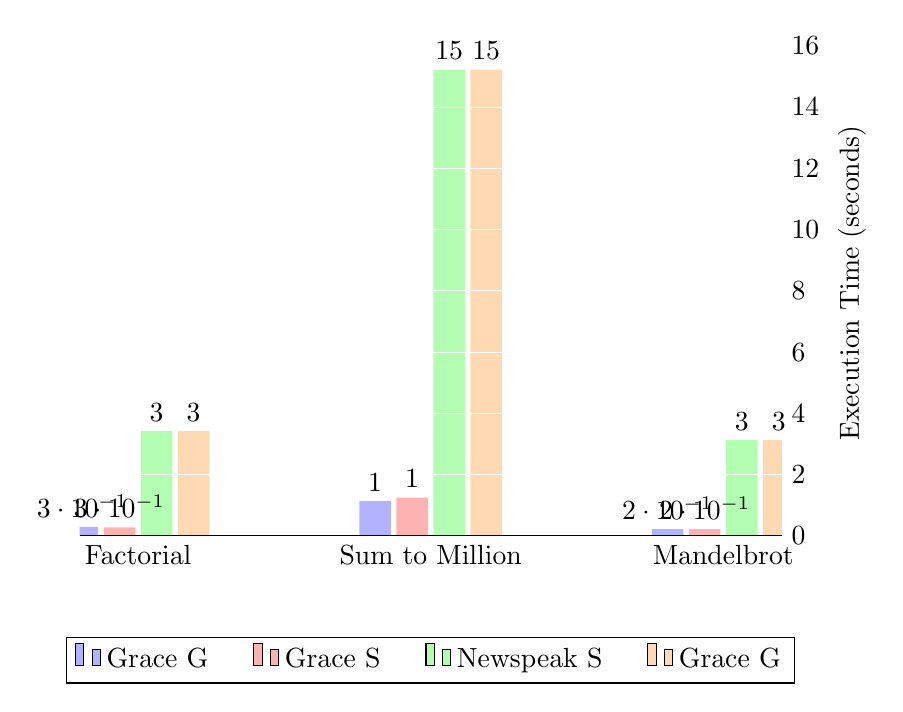
\begin{tikzpicture}
    \begin{axis}[
        ybar, axis on top,
        height=8cm, width=10.5cm,
        bar width=0.4cm,
        ymajorgrids, tick align=inside,
        major grid style={draw=white},
        enlarge y limits={value=.1,upper},
        ymin=0, ymax=15,
        axis x line*=bottom,
        axis y line*=right,
        y axis line style={opacity=0},
        tickwidth=0pt,
        enlarge x limits=true,
        legend style={
            at={(0.5,-0.2)},
            anchor=north,
            legend columns=-1,
            /tikz/every even column/.append style={column sep=0.5cm}
        },
        ylabel={Execution Time (seconds)},
        symbolic x coords={
           Factorial,
           Sum to Million,
           Mandelbrot},
       xtick=data,
       nodes near coords={
        \pgfmathprintnumber[precision=0]{\pgfplotspointmeta}
       }
    ]
    \addplot [draw=none, fill=blue!30] coordinates {
      (Factorial, 0.294)
      (Sum to Million, 1.132)
      (Mandelbrot, 0.224) };
    \addplot [draw=none,fill=red!30] coordinates {
      (Factorial,0.274)
      (Sum to Million, 1.253) 
      (Mandelbrot, 0.223)  };
    \addplot [draw=none, fill=green!30] coordinates {
      (Factorial, 3.431)
      (Sum to Million,  15.223) 
      (Mandelbrot, 3.129) };
    \addplot [draw=none, fill=orange!30] coordinates {
      (Factorial, 3.431)
      (Sum to Million,  15.223) 
      (Mandelbrot, 3.129) };

    \legend{Grace G, Grace S, Newspeak S, Grace G}
    \end{axis}
\end{tikzpicture}
        }
    }
    \caption{The execution time reported by \SOMns{} when executing three integer-based benchmarks: calculating the factorial of 100, calculating the sum the natural numbers from zero up to one million, and calculating $500$ interations of the mandelbrot fractal. The implementations of these benchmarks in \Grace{} and \Newspeak{} have only negliable differences. The table depicts the average execution time over $1000$ iterations, with and without the \Graal{} optimization layer.}
    \label{fig:benchmark}
\end{figure}

Despite being tailored to \Newspeak{}, \SOMns{} can be easily adapted to \Grace{} through our \translator{}. As depicted in \autoref{fig:benchmark}, there is only a marginal loss of performance due to the additional translation step. 
}{}

\section{Conclusion}
\label{s:conclusion}
\iftoggle{introduction}{
    %!TEX root = ../paper.tex

% ---------------------------------------------------------------------------- %
% Outline

\iftoggle{outline}{
    \begin{itemize}
        \item Revisit intro. 
        \item Reconceptualising SOMns as a library for nested OO languages
    \end{itemize}
}{}

\iftoggle{oldcomments}{
	\sm{ok, so, what are the `adaptation mechanisms', the reusable parts you envision so far?
	I would try to give a bit more space to speculating on that, because that's
	likely the part that's most interesting for others.
	%
	Things Truffle doesn't have at the moment is mechanisms to high-level AST manipulation, it doesn't have a notion of lexical scopes, and lexical knowledge.
	Is that something you need for mapping from Grace to SOMns?
	%
	Other aspects missing are libraries for storage strategies for collections (they got them for RPython)
	or things like ropes for strings (immutable tree-like representation, to minimize memory use).
	Libraries of basic math nodes/specializations, assuming that the numeric models
	would be similar between languages (which they are only superficially).
	In terms of standard control structures, it has support for loops.
	Others might be useful, because one typically adds profiling for performance.
	This would make basic steps for language implementers easy.
	%
	Perhaps you have other ideas/aspects you see currently as important.
	}
	\sm{at the moment, I am not sure we fit actually more related work in here.
	Let's not go overboard with the text length.}
}

% 
% ---------------------------------------------------------------------------- %



% ---------------------------------------------------------------------------- %
%

Before the adapted \VM/ is compliant with Grace's semantics, we must address the differences in lexical scoping between Grace (classes can be nested anywhere) and Newspeak (classes can only be nested inside of other classes). As Truffle does not support higher-level \AST/ manipulation or lexical scoping, we are left with the choice of reimplementing new \AST/ nodes using Truffle (a significant amount of work) or otherwise changing the SOMns \AST/ nodes (which may conflict with Newspeak semantics). While language implementation frameworks provide significant advantages, we believe that a set of simple-but-extensible mechanisms for higher-level \AST/ manipulation, lexical scoping, storage strategies would encourage adaption over reimplementation. Through continuing to adapt SOMns for Grace we pursue the development of such mechanisms. If successful, we can begin to reconceptualize the process of language implementation, where developers reuse small but valid \VMs/ with only minor adaption required to implement semantically correct and fast interpreters for their languages.

%
% ---------------------------------------------------------------------------- %


}{}

\iftoggle{appendices}{
    \appendix
    \section{Appendix Title}
}{}

\iftoggle{acknowledge}{
    \acks
    %!TEX root = ../paper.tex

Stefan Marr was funded by a grant of the Austrian
Science Fund (FWF), project number I2491-N31.
}{}


%
% ---------------------------------------------------------------------------- %






% ---------------------------------------------------------------------------- %
% Tail


\bibliographystyle{abbrvnat}
\bibliography{refs/main}



\end{document}


% 
% ---------------------------------------------------------------------------- %

